\section{Обработка данных}
	В результате вычислений, которые заняли примерно месяц, были полученные $.dat$ файлы. Каждый из этих массивов данных соответствует определённому временному шагу. Для последующей обработки и на их основе построение графиков использовалось встроенное средство ANSYS CFD-Post. Для анализа влияния вихрегенераторов на локальное трение и перенос использовались различные сечения в разных частях канала. Некоторые из них представлены на рисунке \ref{fig:planesforanalysis}. 
	\begin{figure}[H]
		\centering
		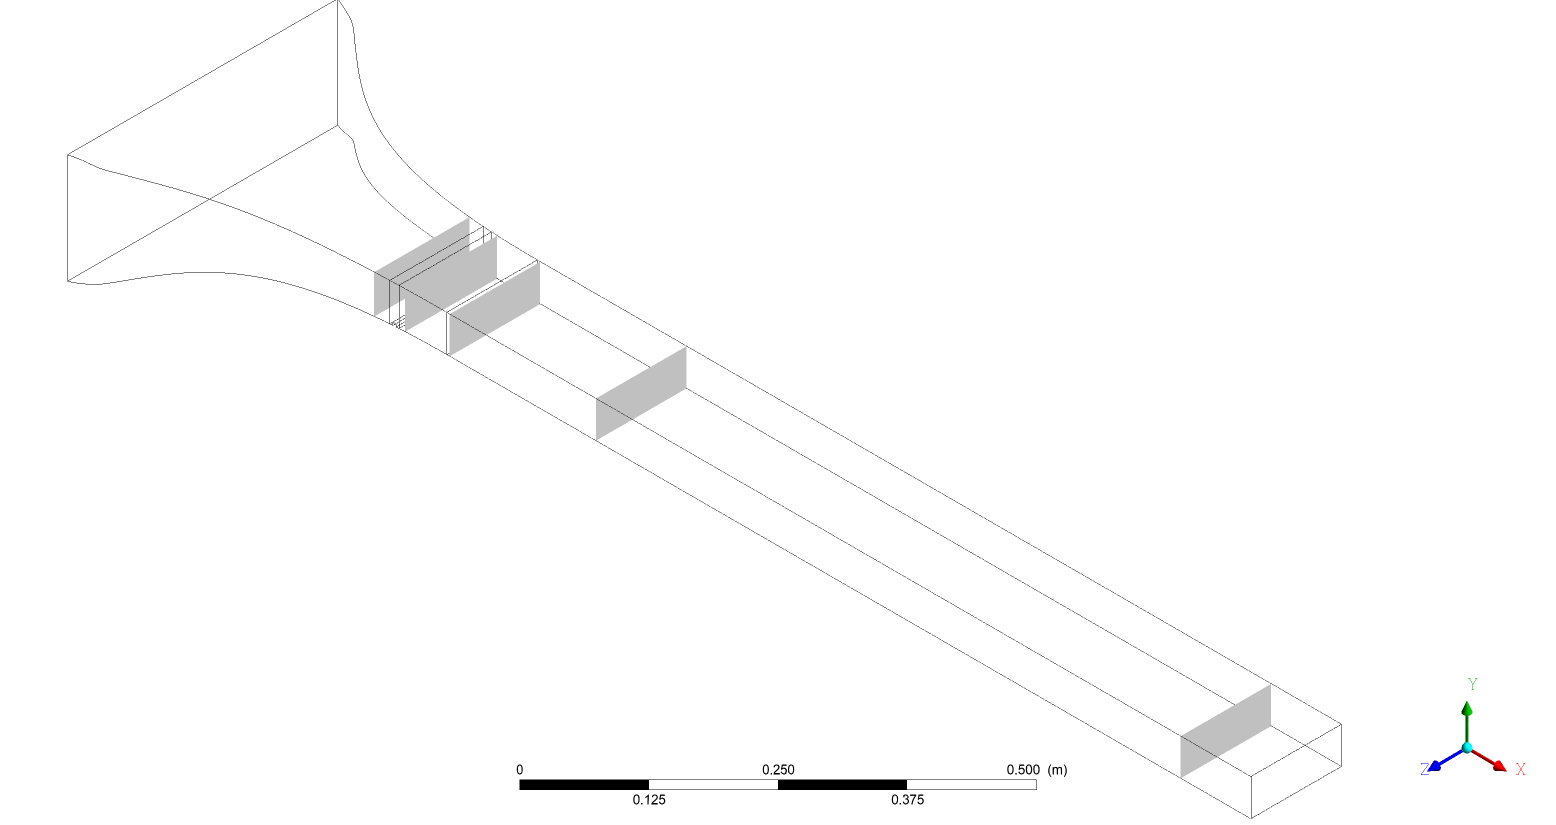
\includegraphics[width=0.9\linewidth]{../Assets/1}
		\caption{Сечения для анализа}
		\label{fig:planesforanalysis}
	\end{figure}
	
	Начало координатных осей модели расположено в центре входа канала. Рассматривались сечения на разных высотах вдоль и различных расстояниях от входа в канал. На таблице ниже представлен перечень сечений, расположение и их описание. Изображения в приложениях имеют названия исходя из таблицы. % ??? по человечески написать ??? %
	\begin{table}[H]
		\begin{center}
			\begin{tabular}{|c|c|c|c|}
				\hline
				Подпись & Плоскость & Расположение & Описание\\
				\hline
				PlaneXY & XY & Z = 0 & вдоль всего канала\\
				\hline
				PlaneYZ300 & YZ & X = 300 & перед препятствием\\
				\hline
				PlaneYZ340 & YZ & X = 340 & за проволокой\\
				\hline
				PlaneYZ400 & YZ & X = 400 & на входе в прямой участок\\
				\hline
				PlaneYZ600 & YZ & X = 600 & далее по каналу\\
				\hline
				PlaneYZ1400 & YZ & X = 1400 & на выходе из канала\\
				\hline
				PlaneXZ0 & XZ & Y = 0 & над пограничным слоем\\
				\hline
				PlaneXZ20M & XZ & Y = -20 & над препятствием\\
				\hline
				PlaneXZ23М & XZ & Y = -23 & на уровне проволоки\\
				\hline
			\end{tabular}
		\end{center}
		\label{tbl:sections}
		\caption{Перечень сечений}
	\end{table}
	
	После окончания вычислений был автоматически сгенерирован график, благодаря которому можно оценить точность полученных результатов на данной сеточной модели. Она достигла значения в $10^{-3}$.
	\begin{figure}[H]
		\centering
		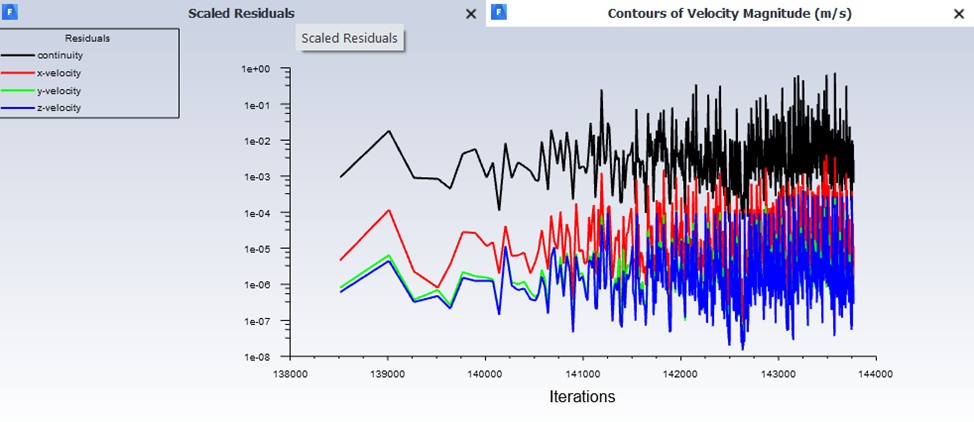
\includegraphics[width=1\linewidth]{../Assets/scaledResiduals}
		\caption{Scaled residuals}
		\label{fig:scaledresiduals}
	\end{figure}
	
\section{Влияние на локальное трение и перенос}
	Далее для удобства описания результатов и их оценка, представлено несколько пунктов по различным параметрам.
\subsection{Скорость}
	Начнём анализ со скорости. По полученным сечениям были построены контуры средних скоростей для различных временных отрезках.
	\begin{figure}[H]
		\centering
		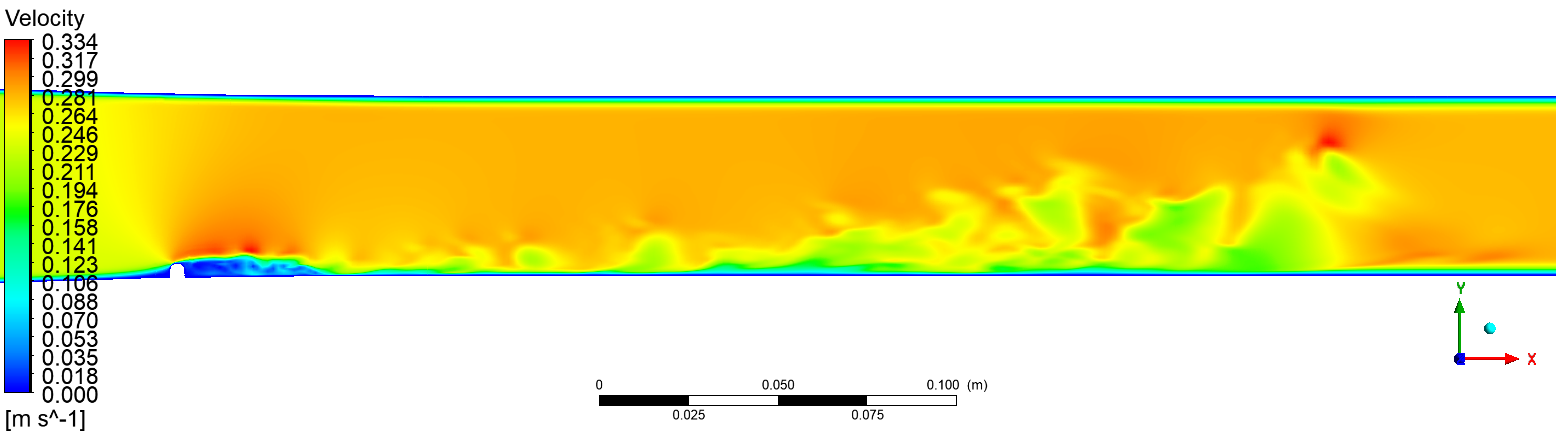
\includegraphics[width=1\linewidth]{../Assets/T16_Velocity_ContourXY}
		\caption{Скорость в продольном сечении XY, t = 1.6 c}
		\label{fig:t16velocitycontourxy}
	\end{figure}
	Как видно из рисунка вдоль канала, скорость сразу за препятствием и на его уровне приблизилась к нулю. А над проволокой значительно увеличилась. Из-за таких резких изменений скорости происходит образование вихревых структур, скорость которых хорошо заметна на этих изображениях.
	
	\begin{figure}[H]
		\begin{subfigure}{.5\textwidth}
			\centering
			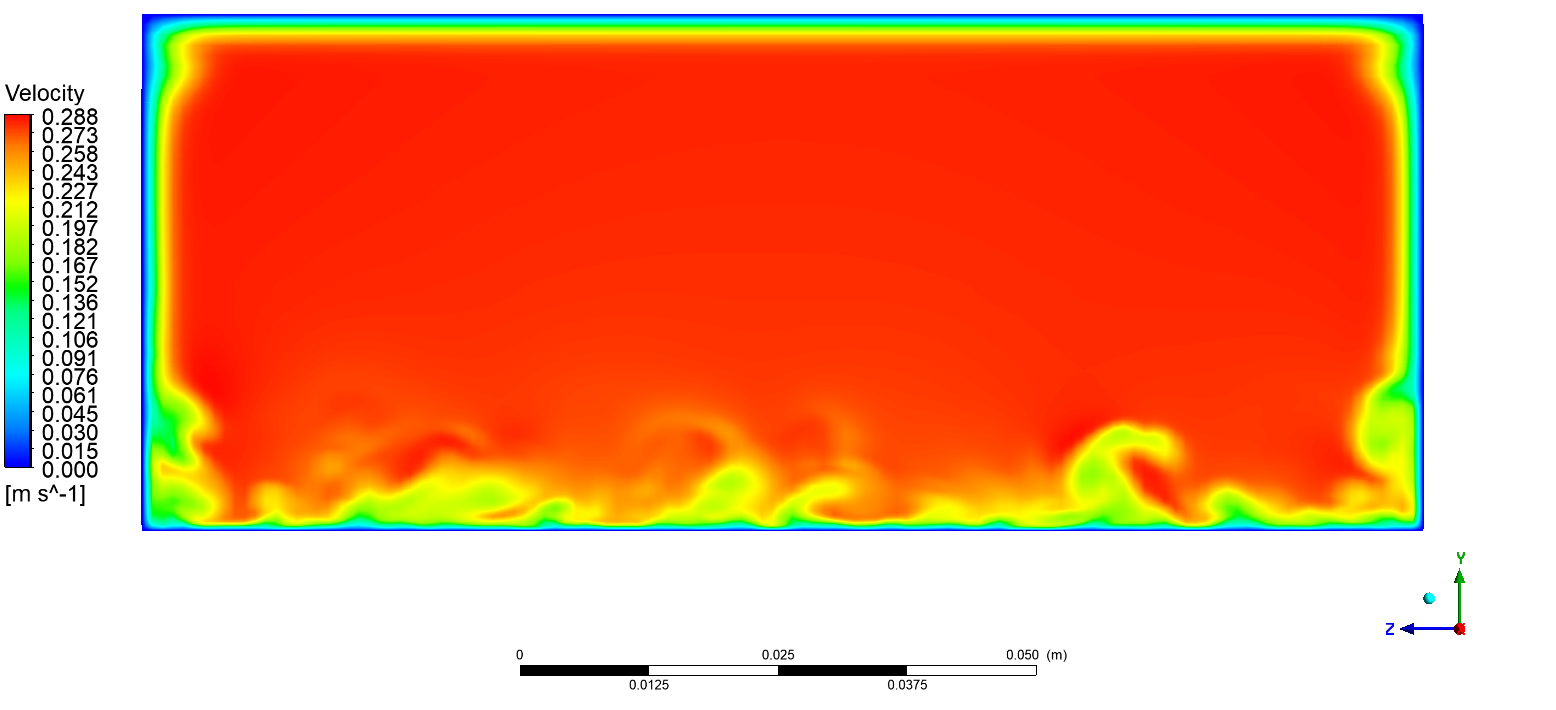
\includegraphics[width=1.1\linewidth]{../Assets/T16_Velocity_ContourYZ400}
			\caption{PlaneYZ400}
			\label{fig:T16VelocityContourYZ340}
		\end{subfigure}%
		\begin{subfigure}{.5\textwidth}
			\centering
			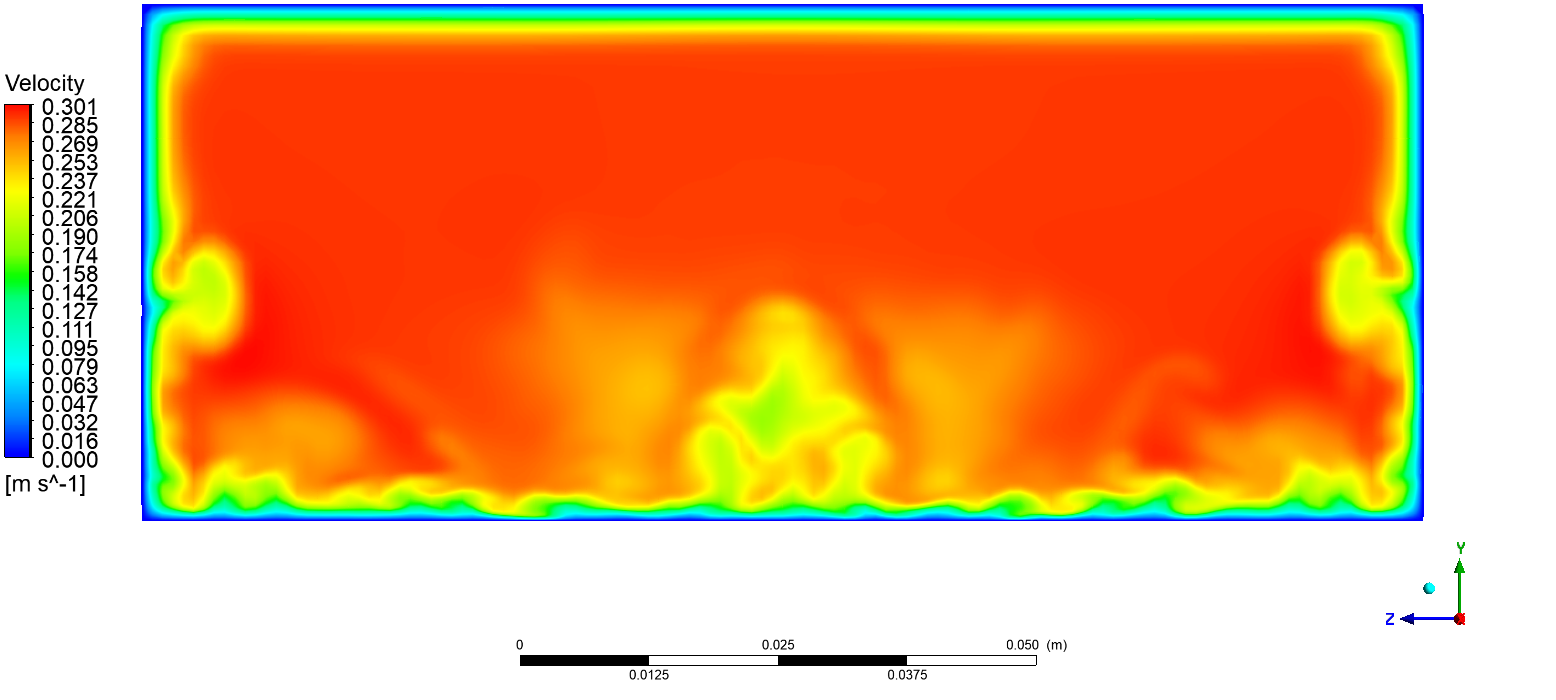
\includegraphics[width=1.1\linewidth]{../Assets/T16_Velocity_ContourYZ600}
			\caption{PlaneYZ600}
			\label{fig:T16VelocityContourYZ400}
		\end{subfigure}
		\caption{Скорость в поперечных сечениях при t = 1.6 с}
		\label{fig:T16VelocityContourYZ}
	\end{figure}
	Эти вихревые образования можно заметить и на рисунке \ref{fig:T16VelocityContourYZ}. 
	
	\begin{figure}[H]
		\centering
		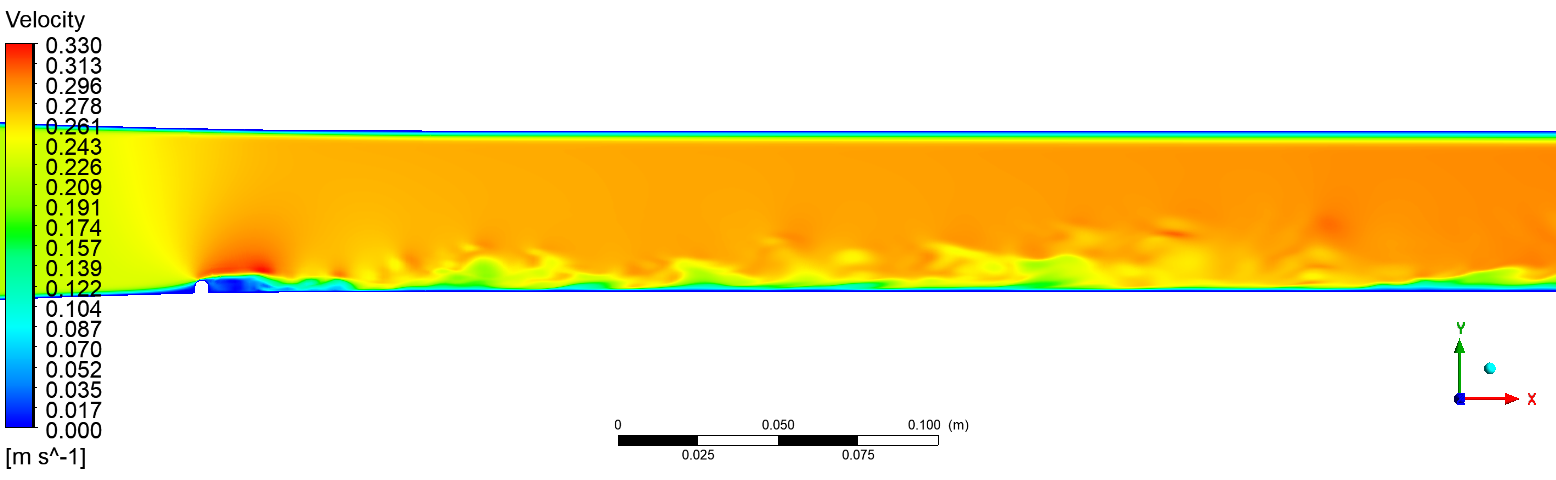
\includegraphics[width=1\linewidth]{../Assets/T96_Velocity_ContourXY}
		\caption{Скорость в продольном сечении XY, t = 9.6 с}
		\label{fig:t96velocitycontourxy}
	\end{figure}
	К моменту времени t = 9.6 с вихревая структура канала стала менее выраженной и крупные вихри преобразовались в мелкие. 
	Рассмотрим подробнее скорость в поперечных сечениях в момент времени t = 9.6 с.
	\begin{figure}[H]
		\begin{subfigure}{.5\textwidth}
			\centering
			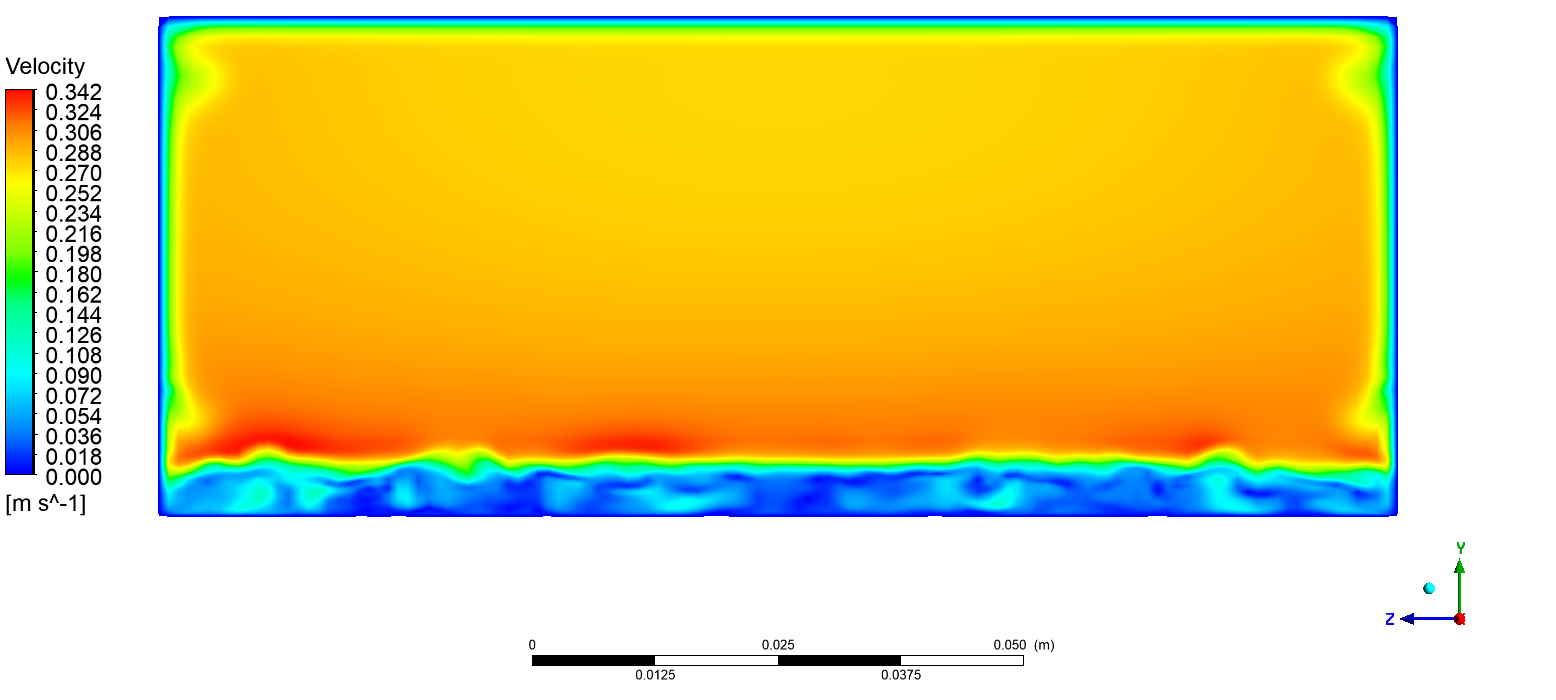
\includegraphics[width=1.1\linewidth]{../Assets/T96_Velocity_ContourYZ340}
			\caption{PlaneYZ340}
			\label{fig:T96VelocityContourYZ340}
		\end{subfigure}%
		\begin{subfigure}{.5\textwidth}
			\centering
			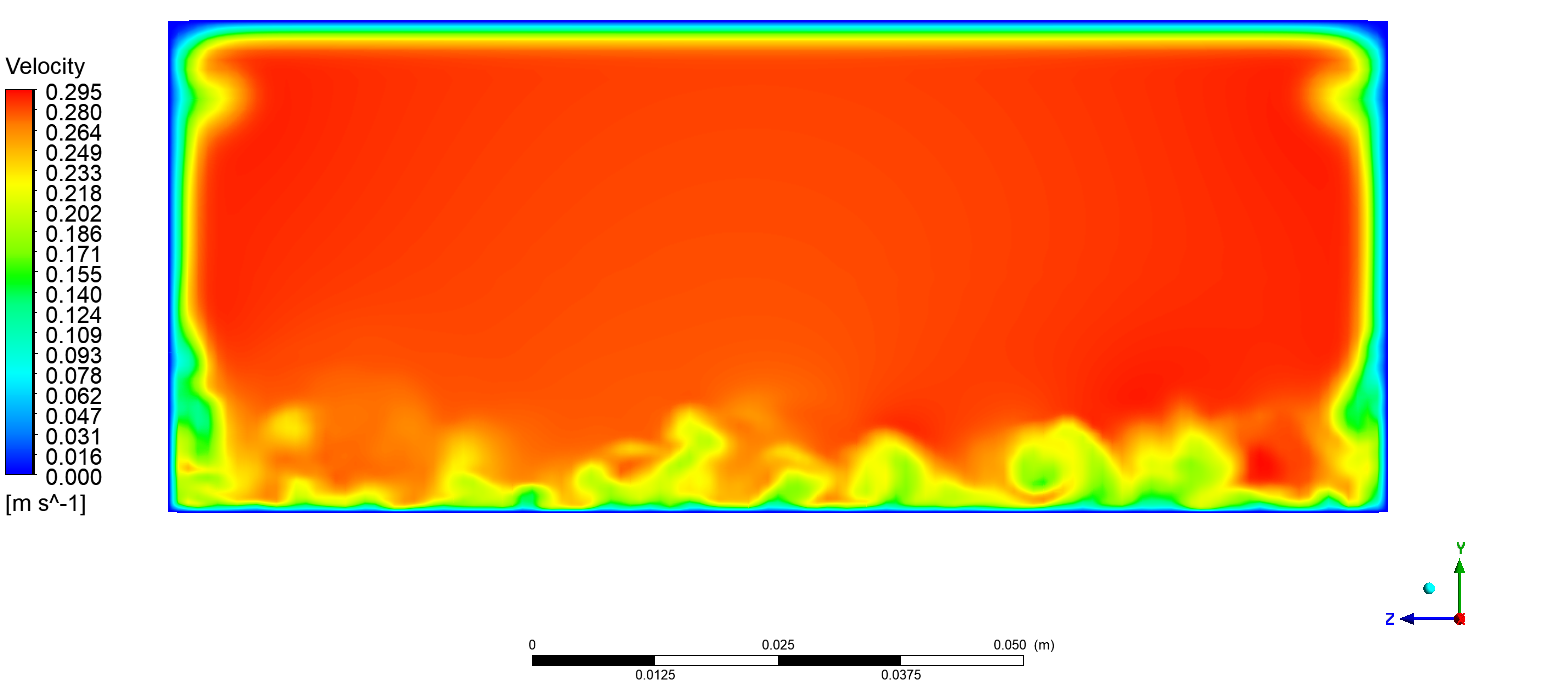
\includegraphics[width=1.1\linewidth]{../Assets/T96_Velocity_ContourYZ400}
			\caption{PlaneYZ400}
			\label{fig:T96VelocityContourYZ400}
		\end{subfigure}
		\\
		\begin{subfigure}{.5\textwidth}
			\centering
			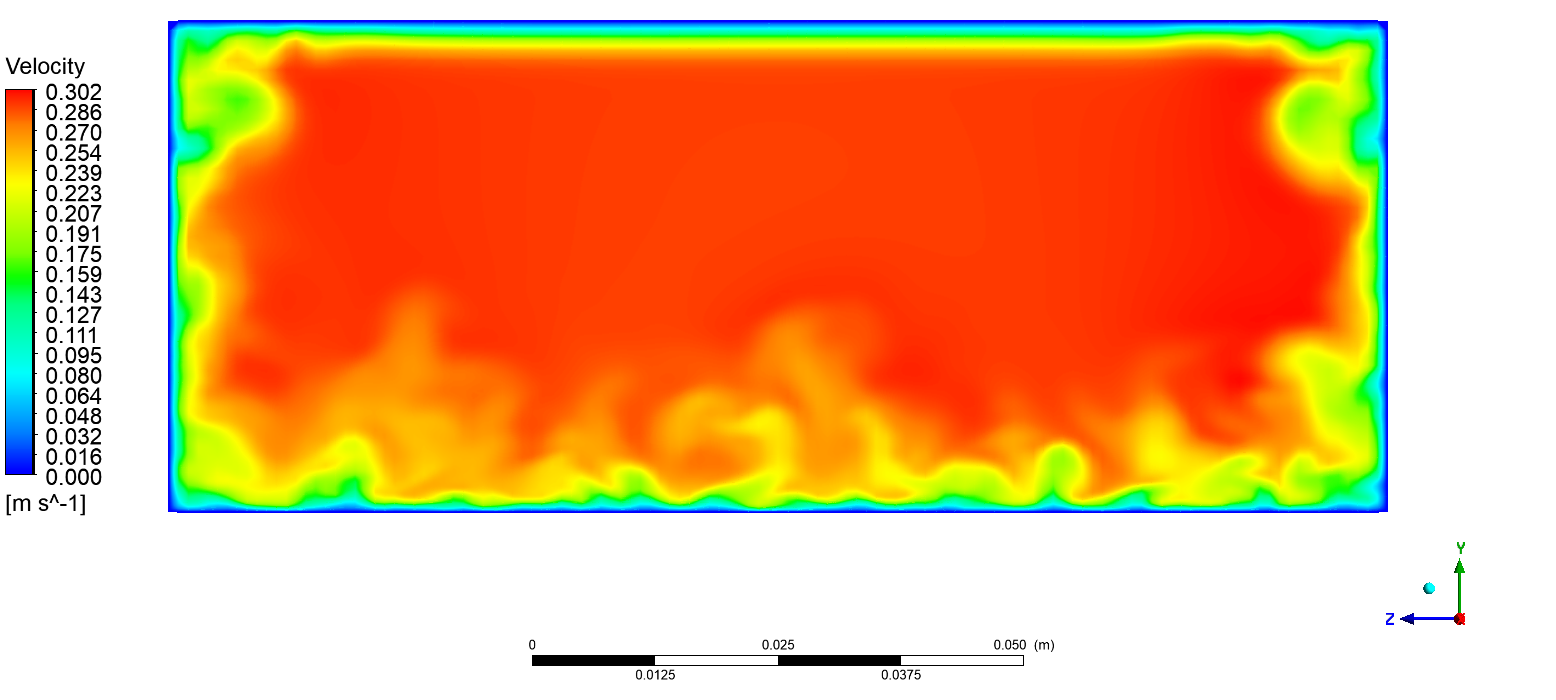
\includegraphics[width=1.1\linewidth]{../Assets/T96_Velocity_ContourYZ600}
			\caption{PlaneYZ600}
			\label{fig:T96VelocityContourYZ600}
		\end{subfigure}%
		\begin{subfigure}{.5\textwidth}
			\centering
			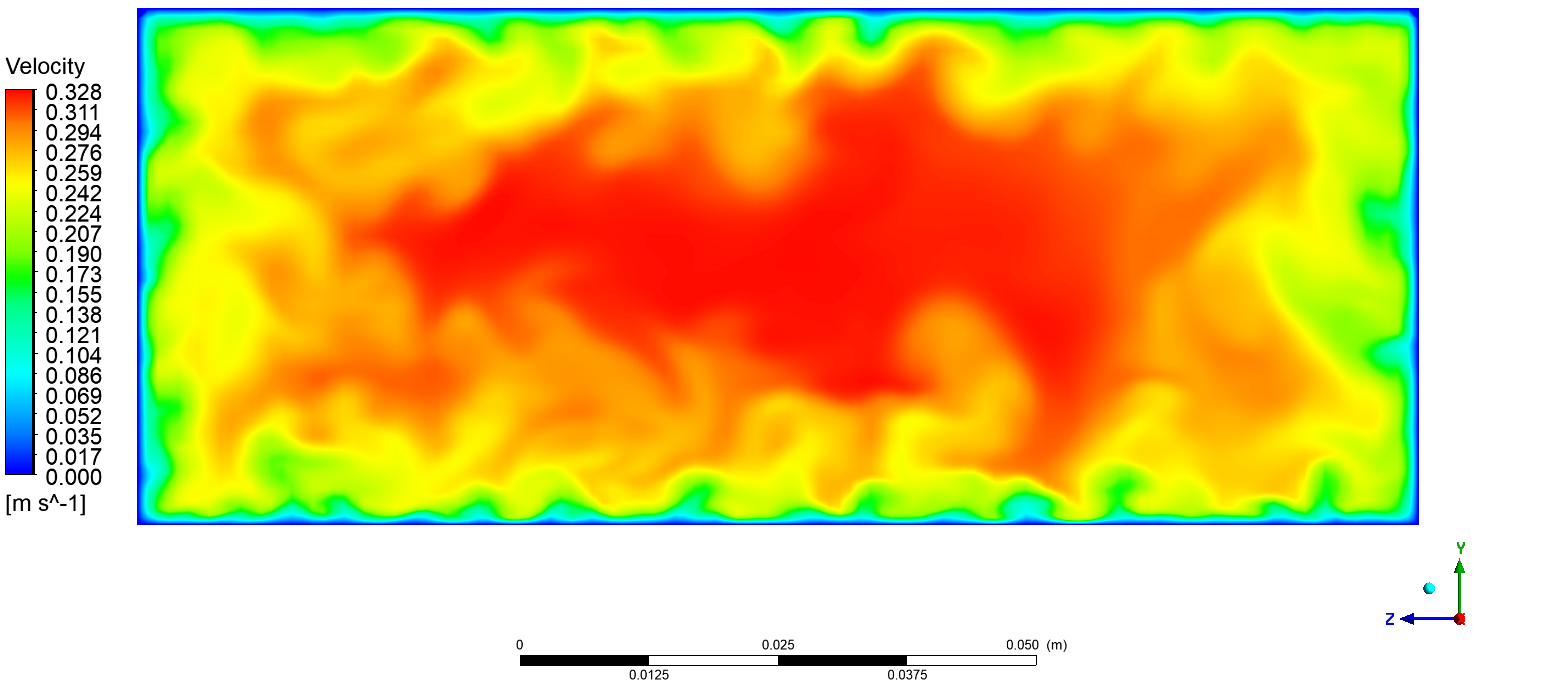
\includegraphics[width=1.1\linewidth]{../Assets/T96_Velocity_ContourYZ1400}
			\caption{PlaneYZ1400}
			\label{fig:T96VelocityContourYZ1400}
		\end{subfigure}
		\caption{Скорость в поперечных сечениях при t = 9.6 с}
		\label{fig:T96VelocityContourYZ}
	\end{figure}
	Как видно на рисунке \ref{fig:T96VelocityContourYZ} образованные вихри постепенно распадаются до вихрей колмагоровского масштаба и диссипируют в энергию.
	
	\begin{figure}[H]
		\begin{subfigure}{1\textwidth}
			\centering
			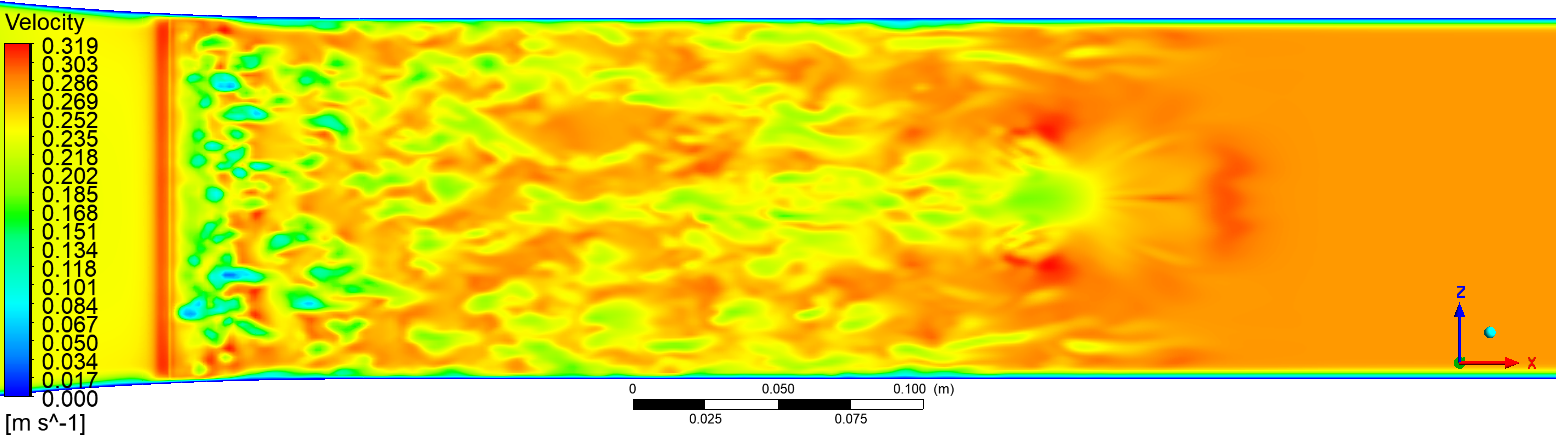
\includegraphics[width=1\linewidth]{../Assets/T16_Velocity_ContourXZ20M}
			\caption{PlaneXZ20M}
			\label{fig:T16VelocityContourXZ20M}
		\end{subfigure}%
		\\
		\begin{subfigure}{1\textwidth}
			\centering
			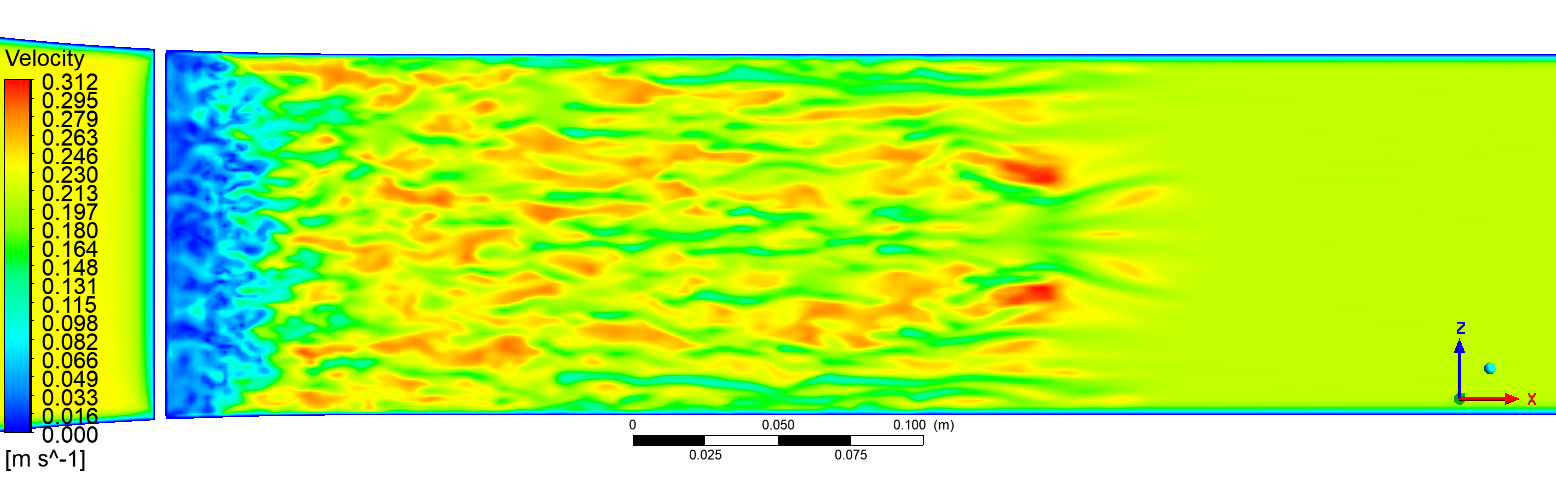
\includegraphics[width=1\linewidth]{../Assets/T16_Velocity_ContourXZ23M}
			\caption{PlaneXZ23M}
			\label{fig:T16VelocityContourXZ23M}
		\end{subfigure}
	 	\caption{Скорость в продольных сечениях XZ при t = 1.6 с}
	 	\label{fig:T16VelocityContourXZ}
	\end{figure}
\subsection{Коэффициент трения}
	Чтобы получить данные коэффициентов трения для построения графиков, в Ansys Fluent были построены необходимые сечения. Они делят канал вдоль на 3 части($z_1 = -31, z_2 = 0, z_3 = 31$). После этого встроенными средствами экспортировались данные в файлы формата $.csv$. Далее при помощи MS Excel были выделены данные касающиеся пограничного слоя. И в конце сгенерированы графики в gnuplot. 
	Оценивались 4 временных отрезка. На графиках отражена зависимость $C_f$ от координаты $x$. При достижении потоком жидкости препятствия происходит резкое изменение $C_f$. Коэффициент вырос в 2.6 раза. По мере продвижения по длине канала коэффициент уменьшался и стабилизировался. Это обусловлено уменьшением влияния вихревых структур на пограничный слой.
	\begin{figure}[H]
		\begin{subfigure}{.5\textwidth}
			\centering
			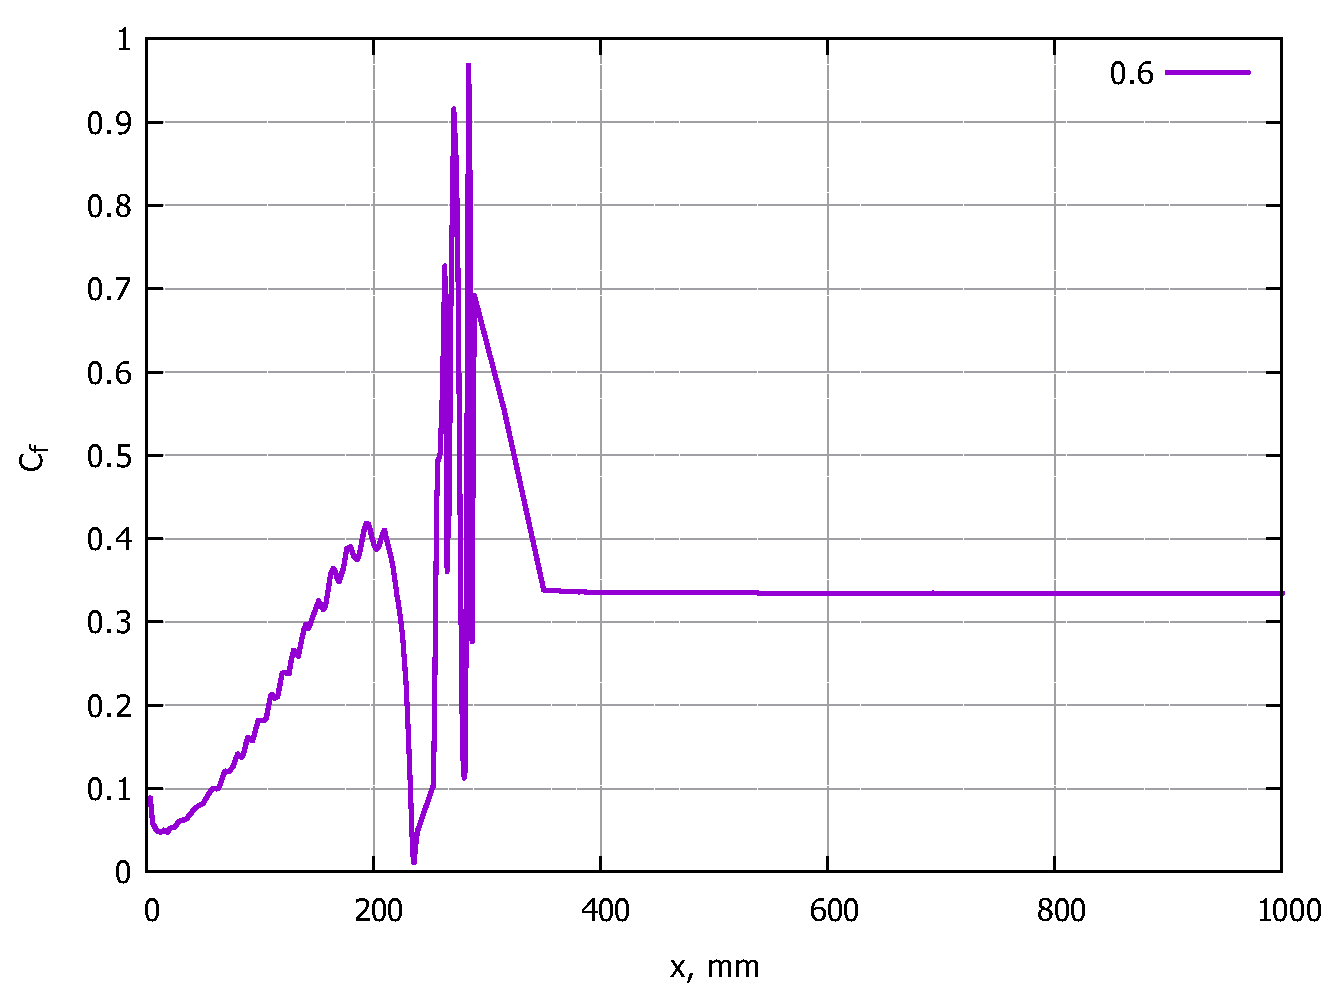
\includegraphics[width=1\linewidth]{../Assets/Cf-T06}
			\caption{t = 0.6 с}
			\label{fig:Cf-T06}
		\end{subfigure}%
		\begin{subfigure}{.5\textwidth}
			\centering
			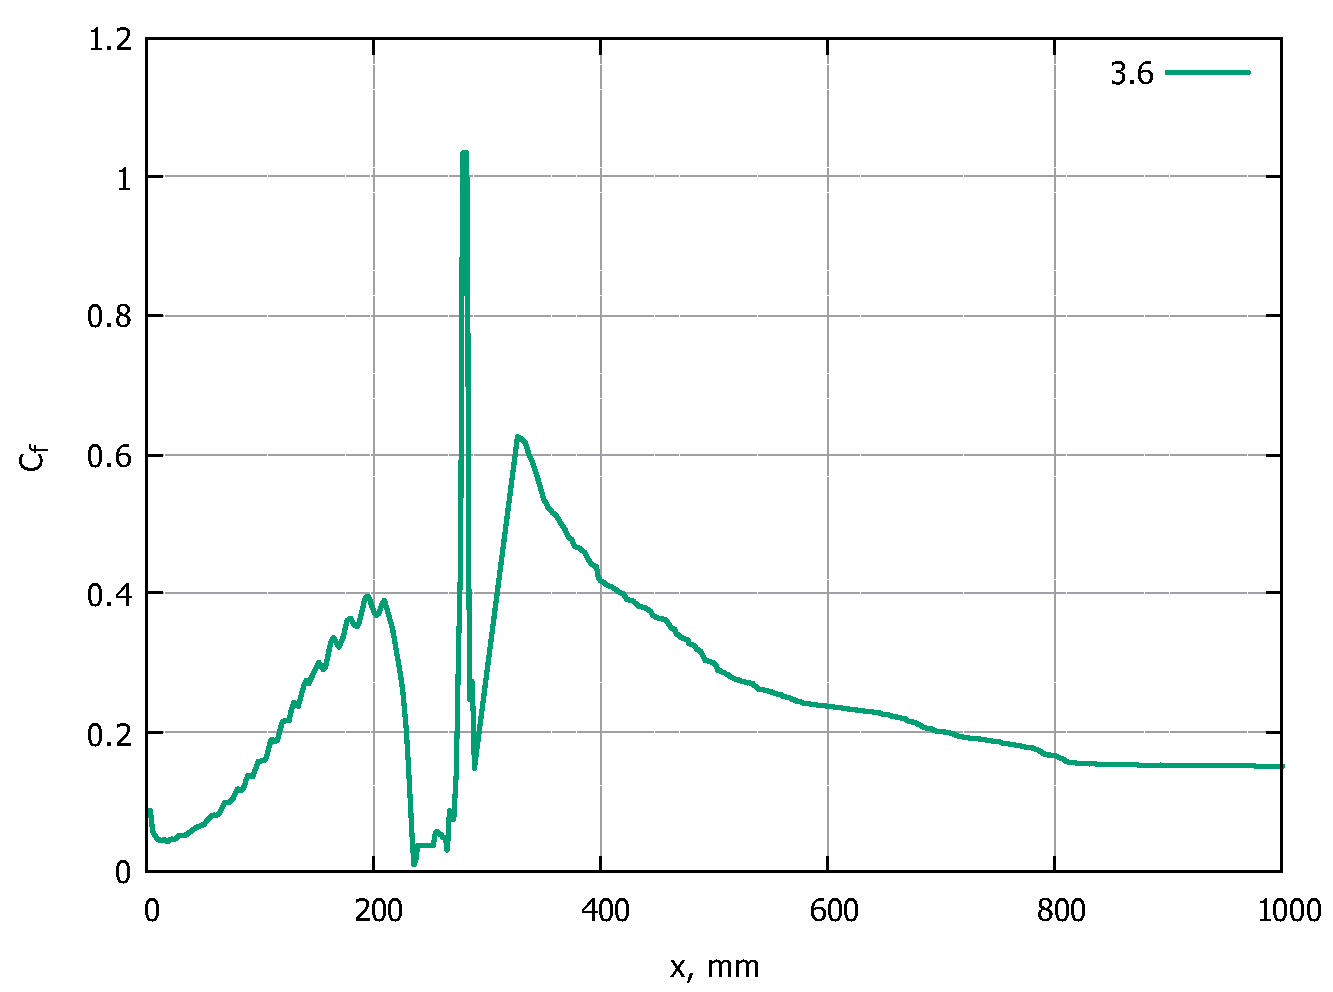
\includegraphics[width=1\linewidth]{../Assets/Cf-T360}
			\caption{t = 3.6 с}
			\label{fig:Cf-T360}
		\end{subfigure}
		\\
		\begin{subfigure}{.5\textwidth}
			\centering
			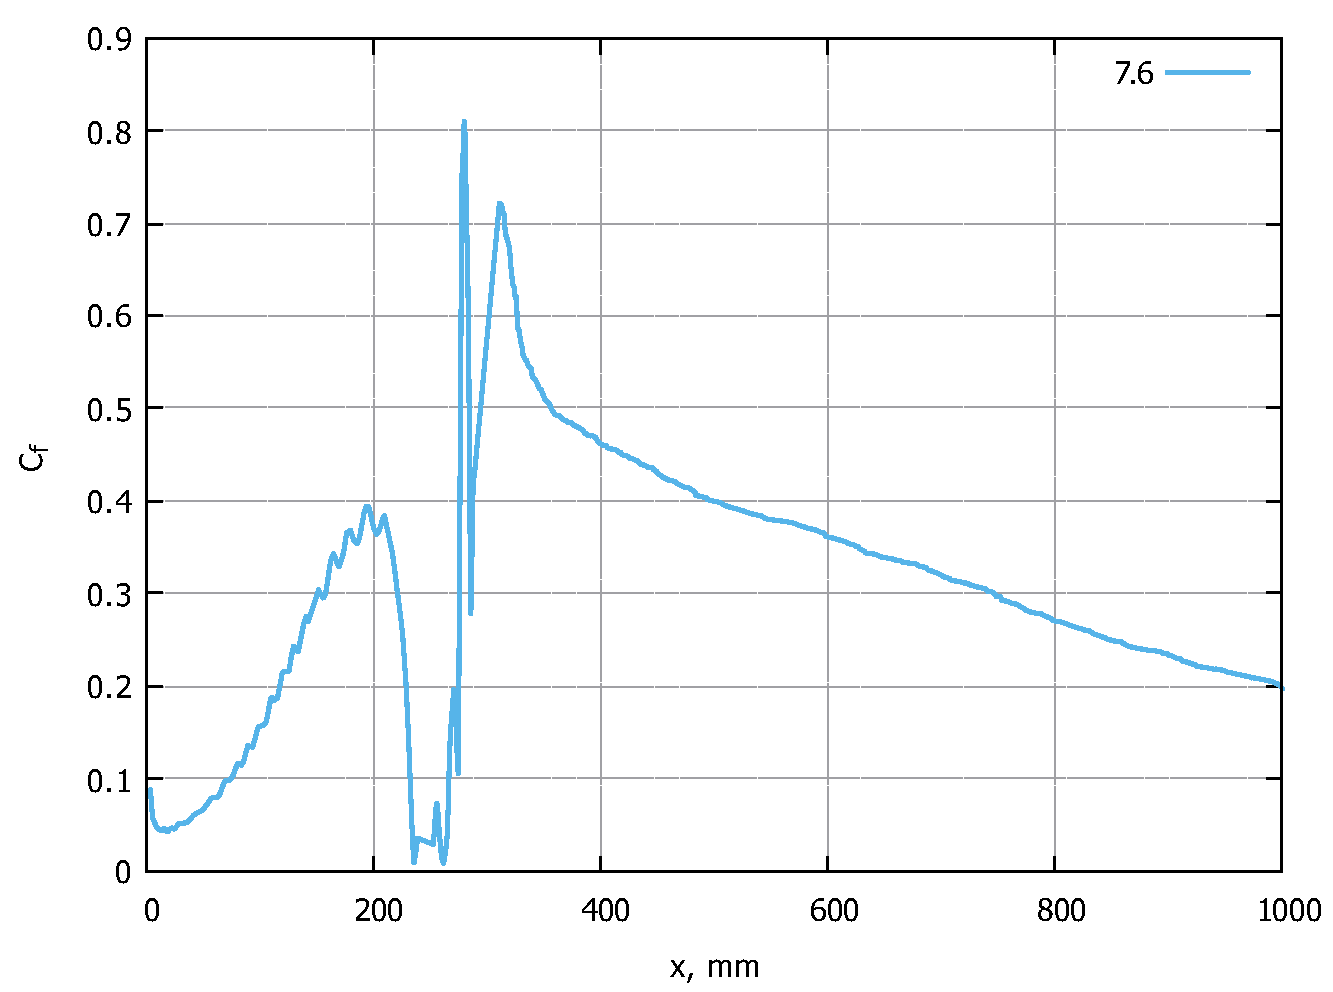
\includegraphics[width=1\linewidth]{../Assets/Cf-T760}
			\caption{t = 7.6 с}
			\label{fig:Cf-T760}
		\end{subfigure}%
		\begin{subfigure}{.5\textwidth}
			\centering
			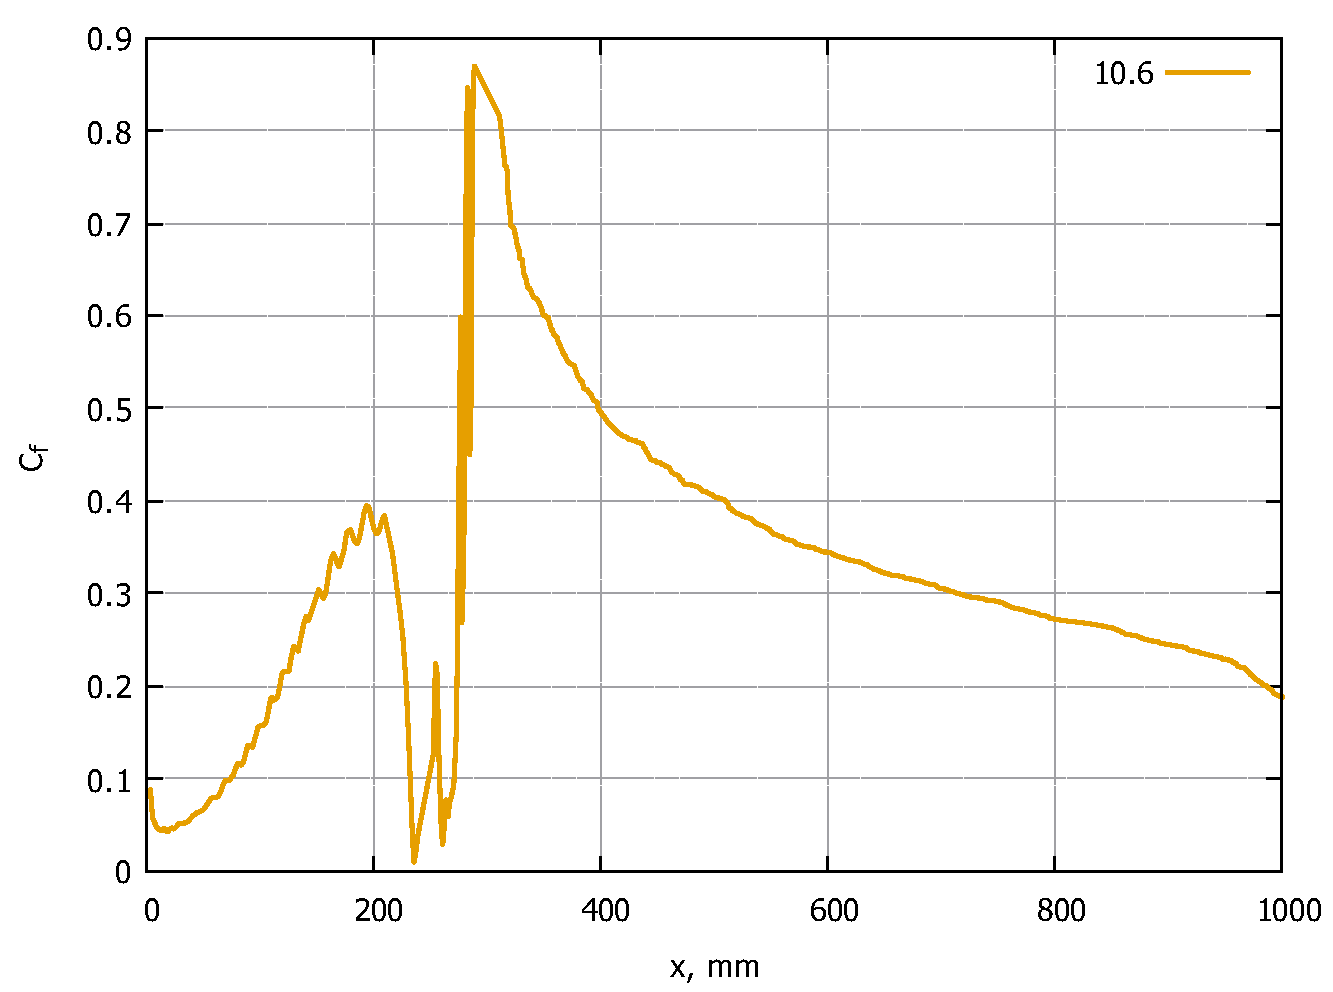
\includegraphics[width=1\linewidth]{../Assets/Cf-T1060}
			\caption{t = 10.6 с}
			\label{fig:Cf-T1060}
		\end{subfigure}
		\caption{Изменение коэффициента трения по длине канала, z = 0}
		\label{fig:cf}
	\end{figure}
\subsection{Q критерий}
	Существуют различные подходы к визуализации вихревых течений, использующие то или иное определение вихря и критерии его идентификации. Классификация методов визуализации вихревых течений проводится в зависимости от того, каким способом определяется вихрь (в области или на линии), является ли метод инвариантным по отношению к преобразованию системы координат, носит подход локальный или глобальный характер\cite{Hunt1988}. Одним из таких является $Q$ критерий($Q-criterion$). Он определяется по двум компонентам: тензор скоростей деформаций $S$ и тензор вращения $\Omega$. 
	\begin{equation}
		S = \frac{1}{2}(\frac{\partial u_i}{\partial x_j} + \frac{\partial u_j}{\partial x_i}) \qquad \Omega = \frac{1}{2}(\frac{\partial u_i}{\partial x_j} - \frac{\partial u_j}{\partial x_i})
	\end{equation}
	Критерий $Q$ определяется как второй инвариант тензора градиента скорости\cite{Wiebel2007}.
	\begin{equation}
		Q = \frac{1}{2}(||\Omega||^2 - ||S||^2)
	\end{equation}
	
	Из этого мы можем видеть, что положительные значения $Q$ указывают на области в поле течения, где преобладает завихренность, а отрицательные значения $Q$ указывают на области, в которых преобладают скорость деформации или вязкое напряжение. Кроме того, существуют различные варианты $Q$ критерия в модифицированных выражениях, которые используются для описания различных областей течения\cite{Berdahl1993,Chong1990}.
	
	% Попробовать отследить его %
	Различные области вихревых образований представлено ниже. На рисунке \ref{fig:q860-t16} можно заметить явно выраженную структуру образовавшегося вихря. 
	\begin{figure}[H]
		\centering
		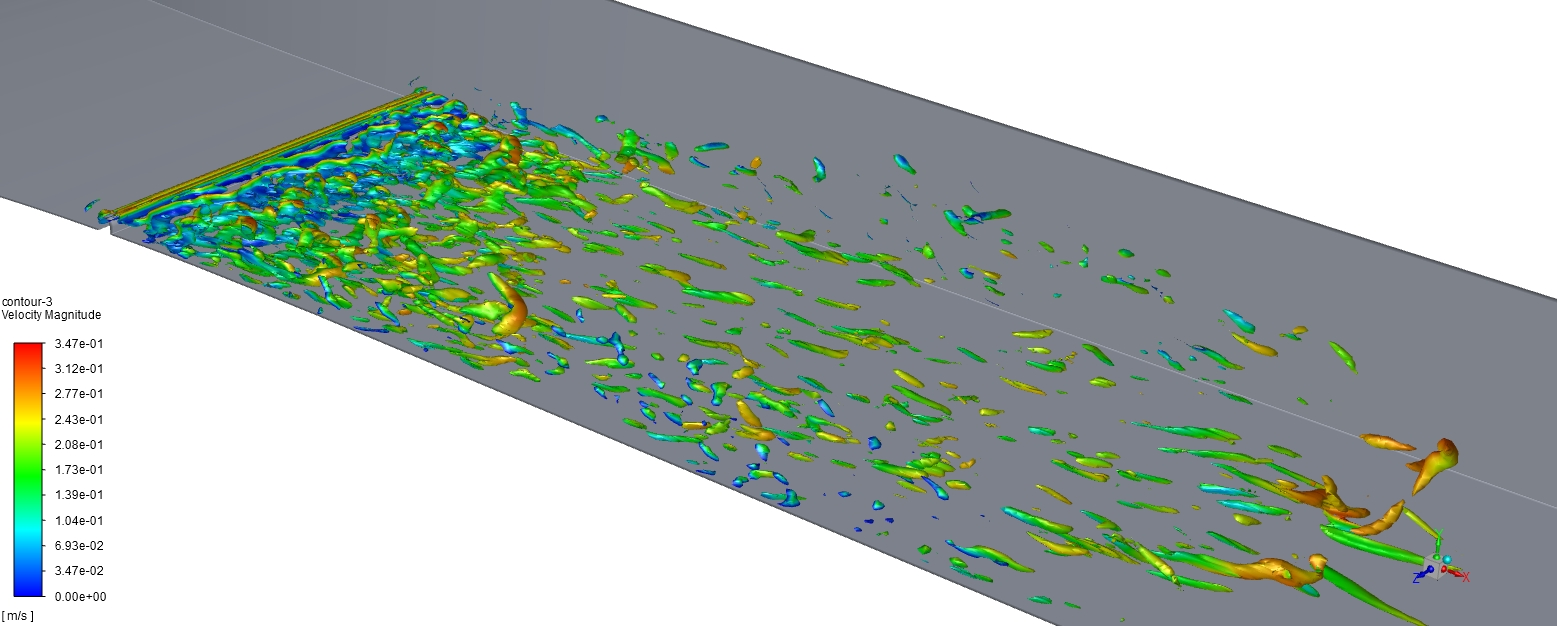
\includegraphics[width=1\linewidth]{../Assets/Q860-t16}
		\caption{Вихревая структура при Q = 860 и t = 1.6 c}
		\label{fig:q860-t16}
	\end{figure}
	\begin{figure}[H]
		\centering
		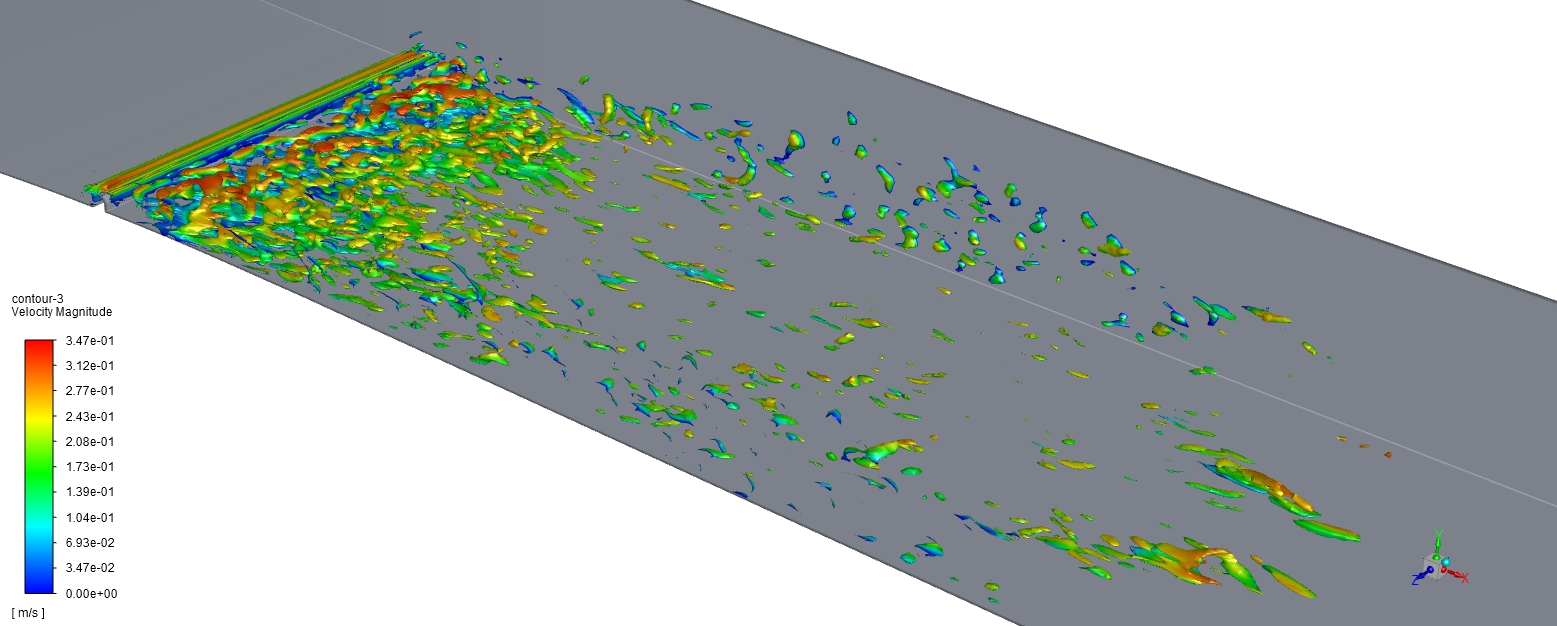
\includegraphics[width=1\linewidth]{../Assets/QM850-t16}
		\caption{Вихревая структура при Q = -850 и t = 1.6 с}
		\label{fig:qm850-t16}
	\end{figure}
	
